\documentclass[twocolumn,a4paper]{article}
\usepackage{fontspec}   %加這個就可以設定字體
\usepackage{xeCJK}       %讓中英文字體分開設置
\usepackage{indentfirst}
\usepackage{listings}
\usepackage[newfloat]{minted}
\usepackage{float}
\usepackage{graphicx}
\usepackage{caption}
\usepackage{fancyhdr}
\usepackage{hyperref}
\usepackage{amsmath}
\usepackage{multirow}
\usepackage[dvipsnames]{xcolor}
\usepackage{graphicx}
\usepackage{tabularx}
\usepackage{booktabs}
\usepackage{caption}
\usepackage{subcaption}
\usepackage{pifont}
\usepackage{amssymb}


\usepackage{pdftexcmds}
\usepackage{catchfile}
\usepackage{ifluatex}
\usepackage{ifplatform}

\usepackage[breakable, listings, skins, minted]{tcolorbox}
\usepackage{etoolbox}
\setminted{fontsize=\footnotesize}
\renewtcblisting{minted}{%
    listing engine=minted,
    minted language=python,
    listing only,
    breakable,
    enhanced,
    minted options = {
        linenos, 
        breaklines=true, 
        breakbefore=., 
        % fontsize=\footnotesize, 
        numbersep=2mm
    },
    overlay={%
        \begin{tcbclipinterior}
            \fill[gray!25] (frame.south west) rectangle ([xshift=4mm]frame.north west);
        \end{tcbclipinterior}
    }   
}

\usepackage[
top=1.5cm,
bottom=0.75cm,
left=1.5cm,
right=1.5cm,
includehead,includefoot,
heightrounded, % to avoid spurious underfull messages
]{geometry} 

\newenvironment{code}{\captionsetup{type=listing}}{}
\SetupFloatingEnvironment{listing}{name=Code}



\title{Visual Recognition using Deep Learning - HW3}
\author{110550088 李杰穎}
\date{\today}


\setCJKmainfont{Noto Serif TC}



\ifwindows
\setmonofont[Mapping=tex-text]{Consolas}
\fi

\XeTeXlinebreaklocale "zh"             %這兩行一定要加,中文才能自動換行
\XeTeXlinebreakskip = 0pt plus 1pt     %這兩行一定要加,中文才能自動換行

\newcommand*{\dif}{\mathop{}\!\mathrm{d}}


%\setlength{\parindent}{0em}
%\setlength{\parskip}{2em}
%\renewcommand{\baselinestretch}{1.25}
%\setlength{\droptitle}{-7.5em}   % This is your set screw
%\setlength{\columnsep}{2em}

\begin{document}
\maketitle
\section{Introduction}

This homework focuses on cell instance segmentation using the Mask R-CNN\cite{he2017mask} framework. The dataset consists of colored medical images containing four types of cells (class1, class2, class3, class4), each with corresponding instance masks. The task requires detecting and segmenting individual cells with high precision, which is crucial for biomedical research and clinical diagnostics. To enhance model performance, I utilize ConvNeXt\cite{liu2022convnet}, a state-of-the-art backbone architecture, combined with advanced data augmentation techniques to overcome the limitation of having only approximately 209 training images.

\section{Method}

\subsection{Data Pre-processing}
The dataset consists of 209 training/validation images and 101 test images in \texttt{.tif} format. Each training image has corresponding instance mask files for four cell classes, with unique pixel values representing individual cell instances. The images were normalized and subjected to extensive data augmentation to increase training data diversity. The augmentation pipeline was designed to preserve the integrity of cell structures while introducing meaningful variations. For each mask image, I extract individual cell instances by identifying unique pixel values, then generate corresponding binary masks and bounding boxes for training the instance segmentation model.

\subsection{Model Architecture}
I implemented a Mask R-CNN architecture with a ConvNeXt-Base\cite{liu2022convnet} backbone to enhance feature extraction capabilities.

\begin{itemize}
    \item \textbf{Backbone:} ConvNeXt-Base, a state-of-the-art CNN architecture that combines the strengths of transformers and CNNs. This backbone delivers superior feature representation compared to traditional ResNet models, with 89M parameters.
    \item \textbf{Neck:} Feature Pyramid Network (FPN)\cite{lin2017feature} to handle multi-scale feature extraction, essential for detecting cells of varying sizes. The FPN creates a feature hierarchy that allows the model to effectively detect both small and large cell instances.
    \item \textbf{Head:} Standard Mask R-CNN heads for classification, bounding box regression, and mask prediction, with hidden layers of 256 dimensions.
    \item \textbf{Input Size:} Original image dimensions preserved to maintain fine details in cellular structures, critical for accurate boundary delineation.
    \item \textbf{Classes:} 5 classes (background + 4 cell types)
\end{itemize}

I integrated the ConvNeXt backbone with the Mask R-CNN framework by creating a custom BackboneWithFPN implementation, which required special attention to stage extraction and return layers mapping for the FPN. This integration process involved carefully aligning the ConvNeXt feature channels with the FPN input requirements to ensure optimal information flow.

\subsection{Advanced Data Augmentation}
To overcome the limitation of having only 209 training images, I implemented an extensive augmentation pipeline using Albumentations:

\begin{code}
\captionof{listing}{\textbf{Implementation of advanced data augmentation pipeline using Albumentations, designed specifically for cell instance segmentation with synchronized transformations for images, masks, and bounding boxes}}
\begin{minted}
A.Compose([
    A.HorizontalFlip(p=0.5),
    A.VerticalFlip(p=0.5),
    A.OneOf([
        A.RandomBrightnessContrast(brightness_limit=0.2, contrast_limit=0.2, p=1.0),
        A.CLAHE(p=1.0),
        A.RandomGamma(p=1.0),
    ], p=0.7),
    A.OneOf([
        A.GaussianBlur(blur_limit=(3, 5), p=1.0),
        A.MedianBlur(blur_limit=5, p=1.0)
    ], p=0.3),
    A.OneOf([
        A.ElasticTransform(alpha=120, sigma=120 * 0.05, p=1.0),
        A.GridDistortion(p=1.0),
        A.OpticalDistortion(distort_limit=2, p=1.0)
    ], p=0.5),
    A.Normalize(mean=[0, 0, 0], std=[1, 1, 1], max_pixel_value=255.0),
    ToTensorV2()
    ], bbox_params=A.BboxParams(
    format='pascal_voc',  # [x1, y1, x2, y2]
    label_fields=['category_ids'],
))
\end{minted}
\end{code}


\subsection{Training Procedure}
We used the following settings for training:
\begin{itemize}
    \item Epochs: 20
    \item Batch size: 2
    \item Optimizer: AdamW with weight decay of 5e-4
    \item Learning rate: 3e-4 with CosineAnnealing scheduler (decreasing to 0)
    \item Loss: Combined losses from RPN, classification, bounding box regression, and mask prediction
\end{itemize}

To prevent overfitting on the limited dataset, I implemented early stopping based on validation mAP and applied strategic GPU memory management to accommodate the large backbone model.

\subsection{Evaluation Metrics}
For evaluation, I used the standard COCO evaluation metrics converted to the proper format using pycocotools\cite{cocoeval2015,lin2014microsoft}:

\begin{itemize}
    \item mAP: Mean Average Precision across IoU thresholds from 0.5 to 0.95
    \item AP50: Average Precision at IoU threshold of 0.5
    \item AP75: Average Precision at IoU threshold of 0.75
\end{itemize}

The model was evaluated on a 5\% validation split of the training data. The best model was selected based on the highest mAP score achieved during training.

\section{Results}

\subsection{Training \& Validation Curve}

\begin{figure}[H]
\centering
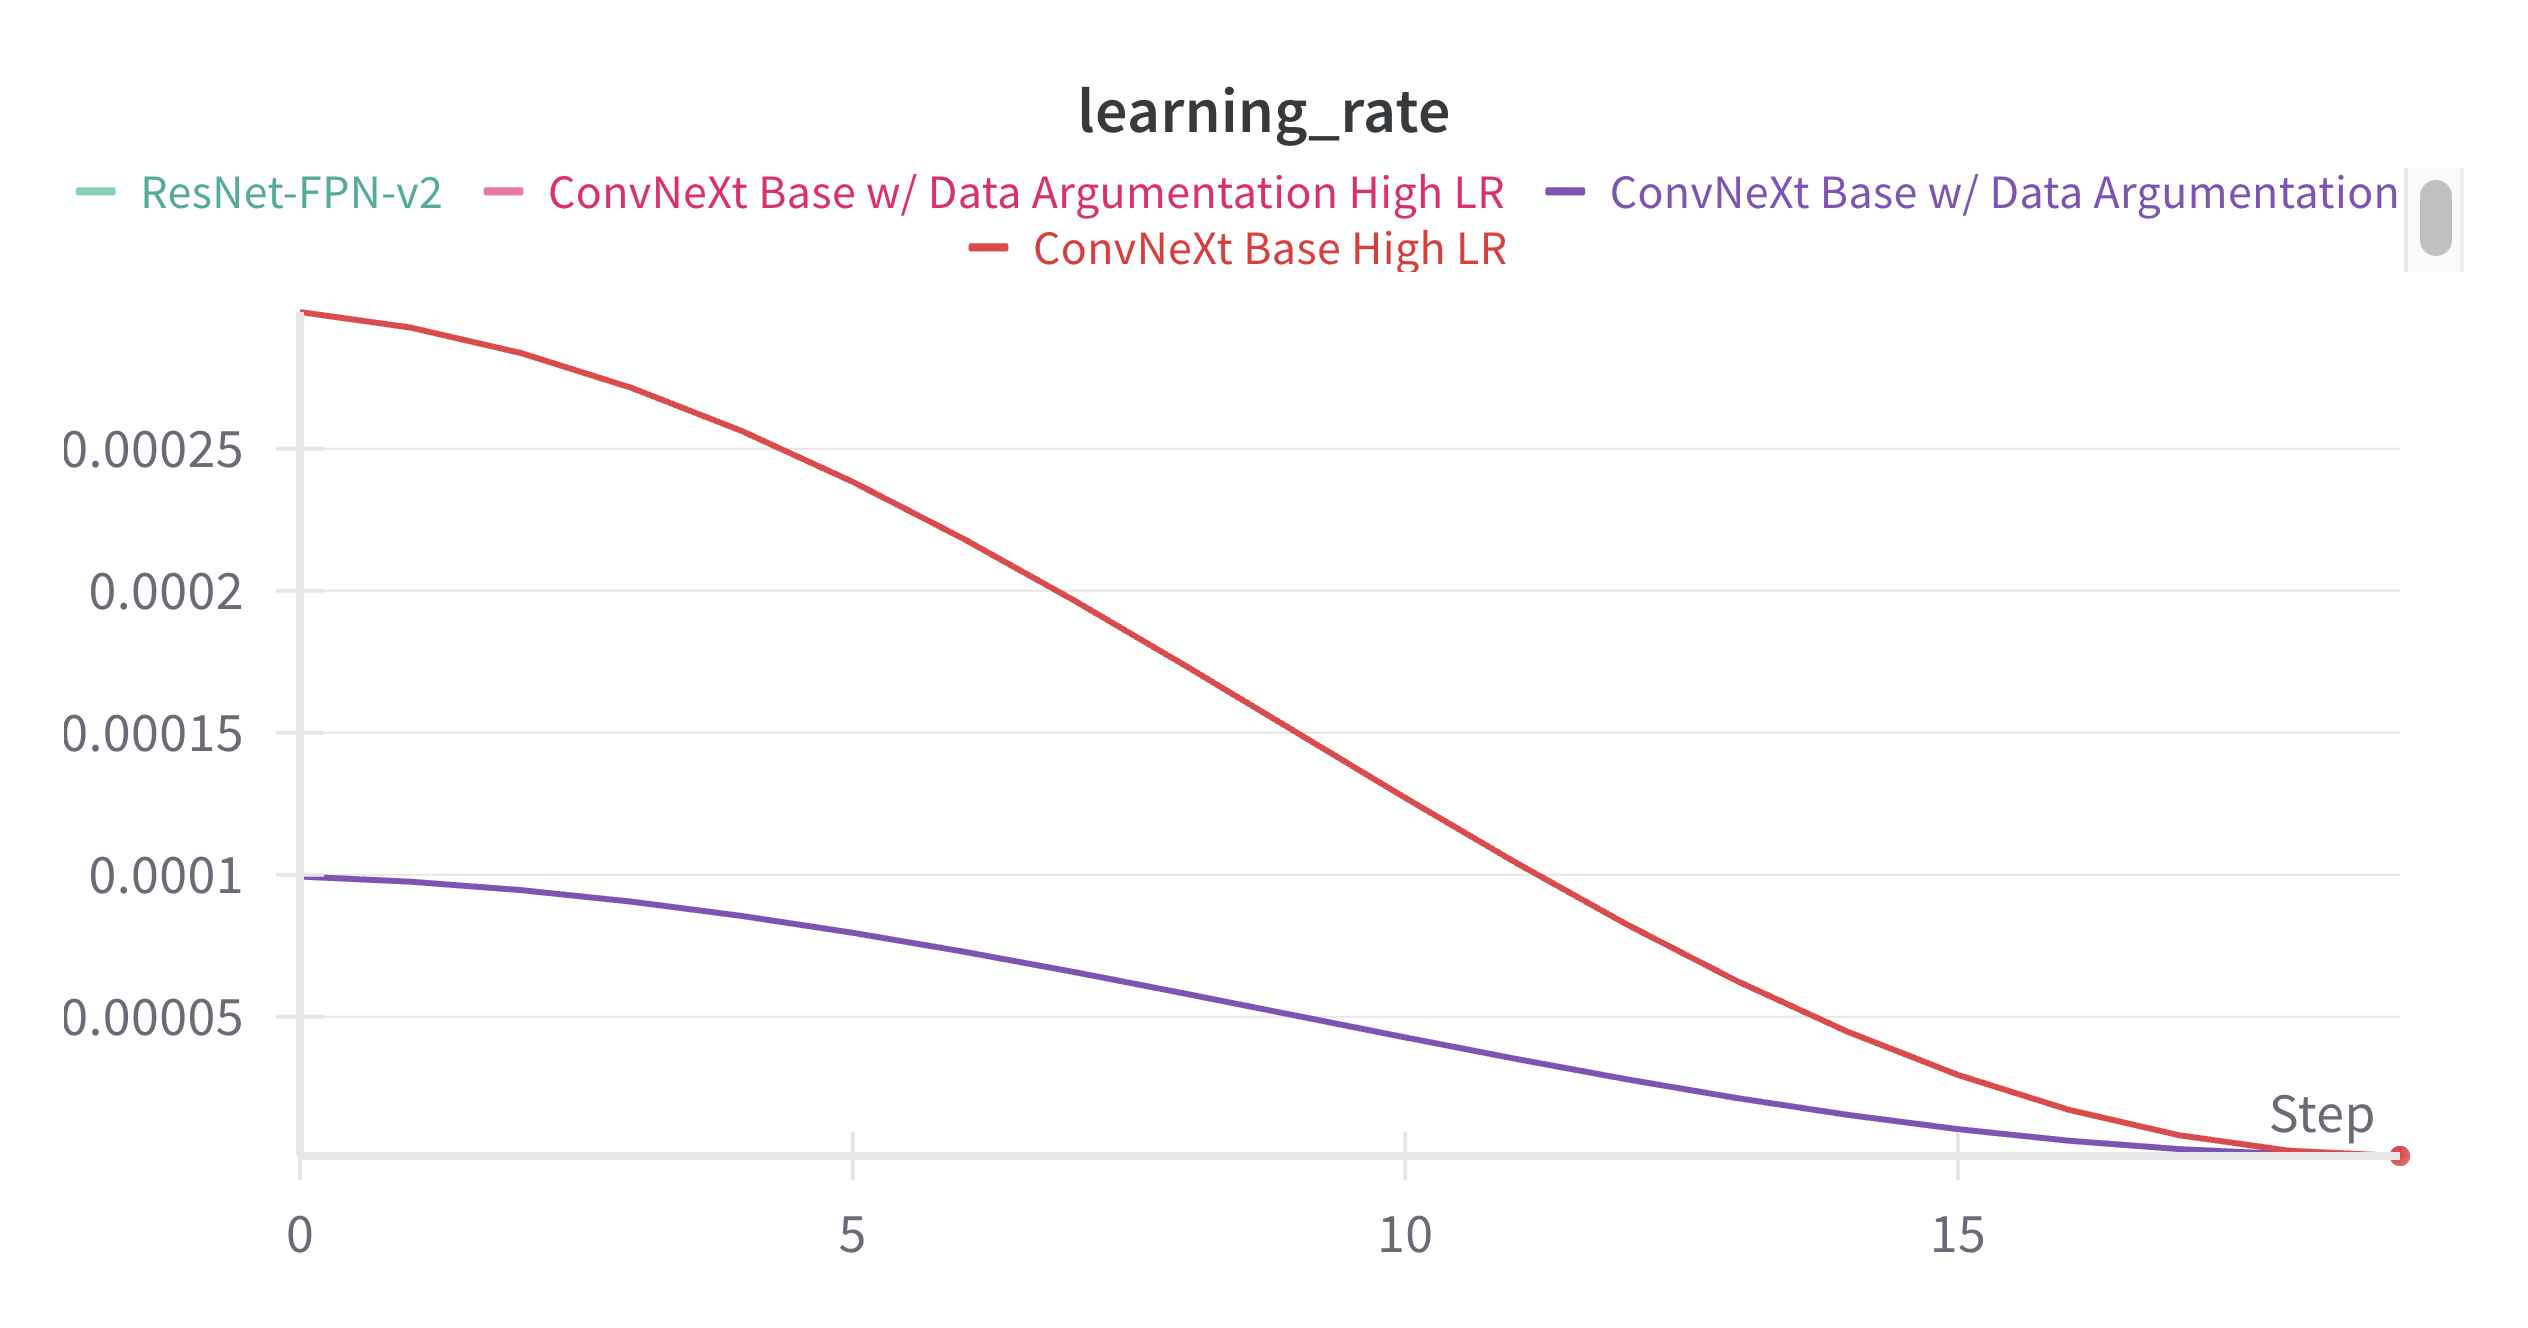
\includegraphics[width=0.95\linewidth]{figs/lr}
\caption{\textbf{Learning rate schedule during training.} The cosine annealing scheduler gradually reduces the learning rate from 3e-4 (or 1e-4) to 0 over 20 epochs, allowing for initial rapid learning followed by fine-tuning of weights in later epochs.}
\label{fig:lr}
\end{figure}

\begin{figure}[H]
\centering
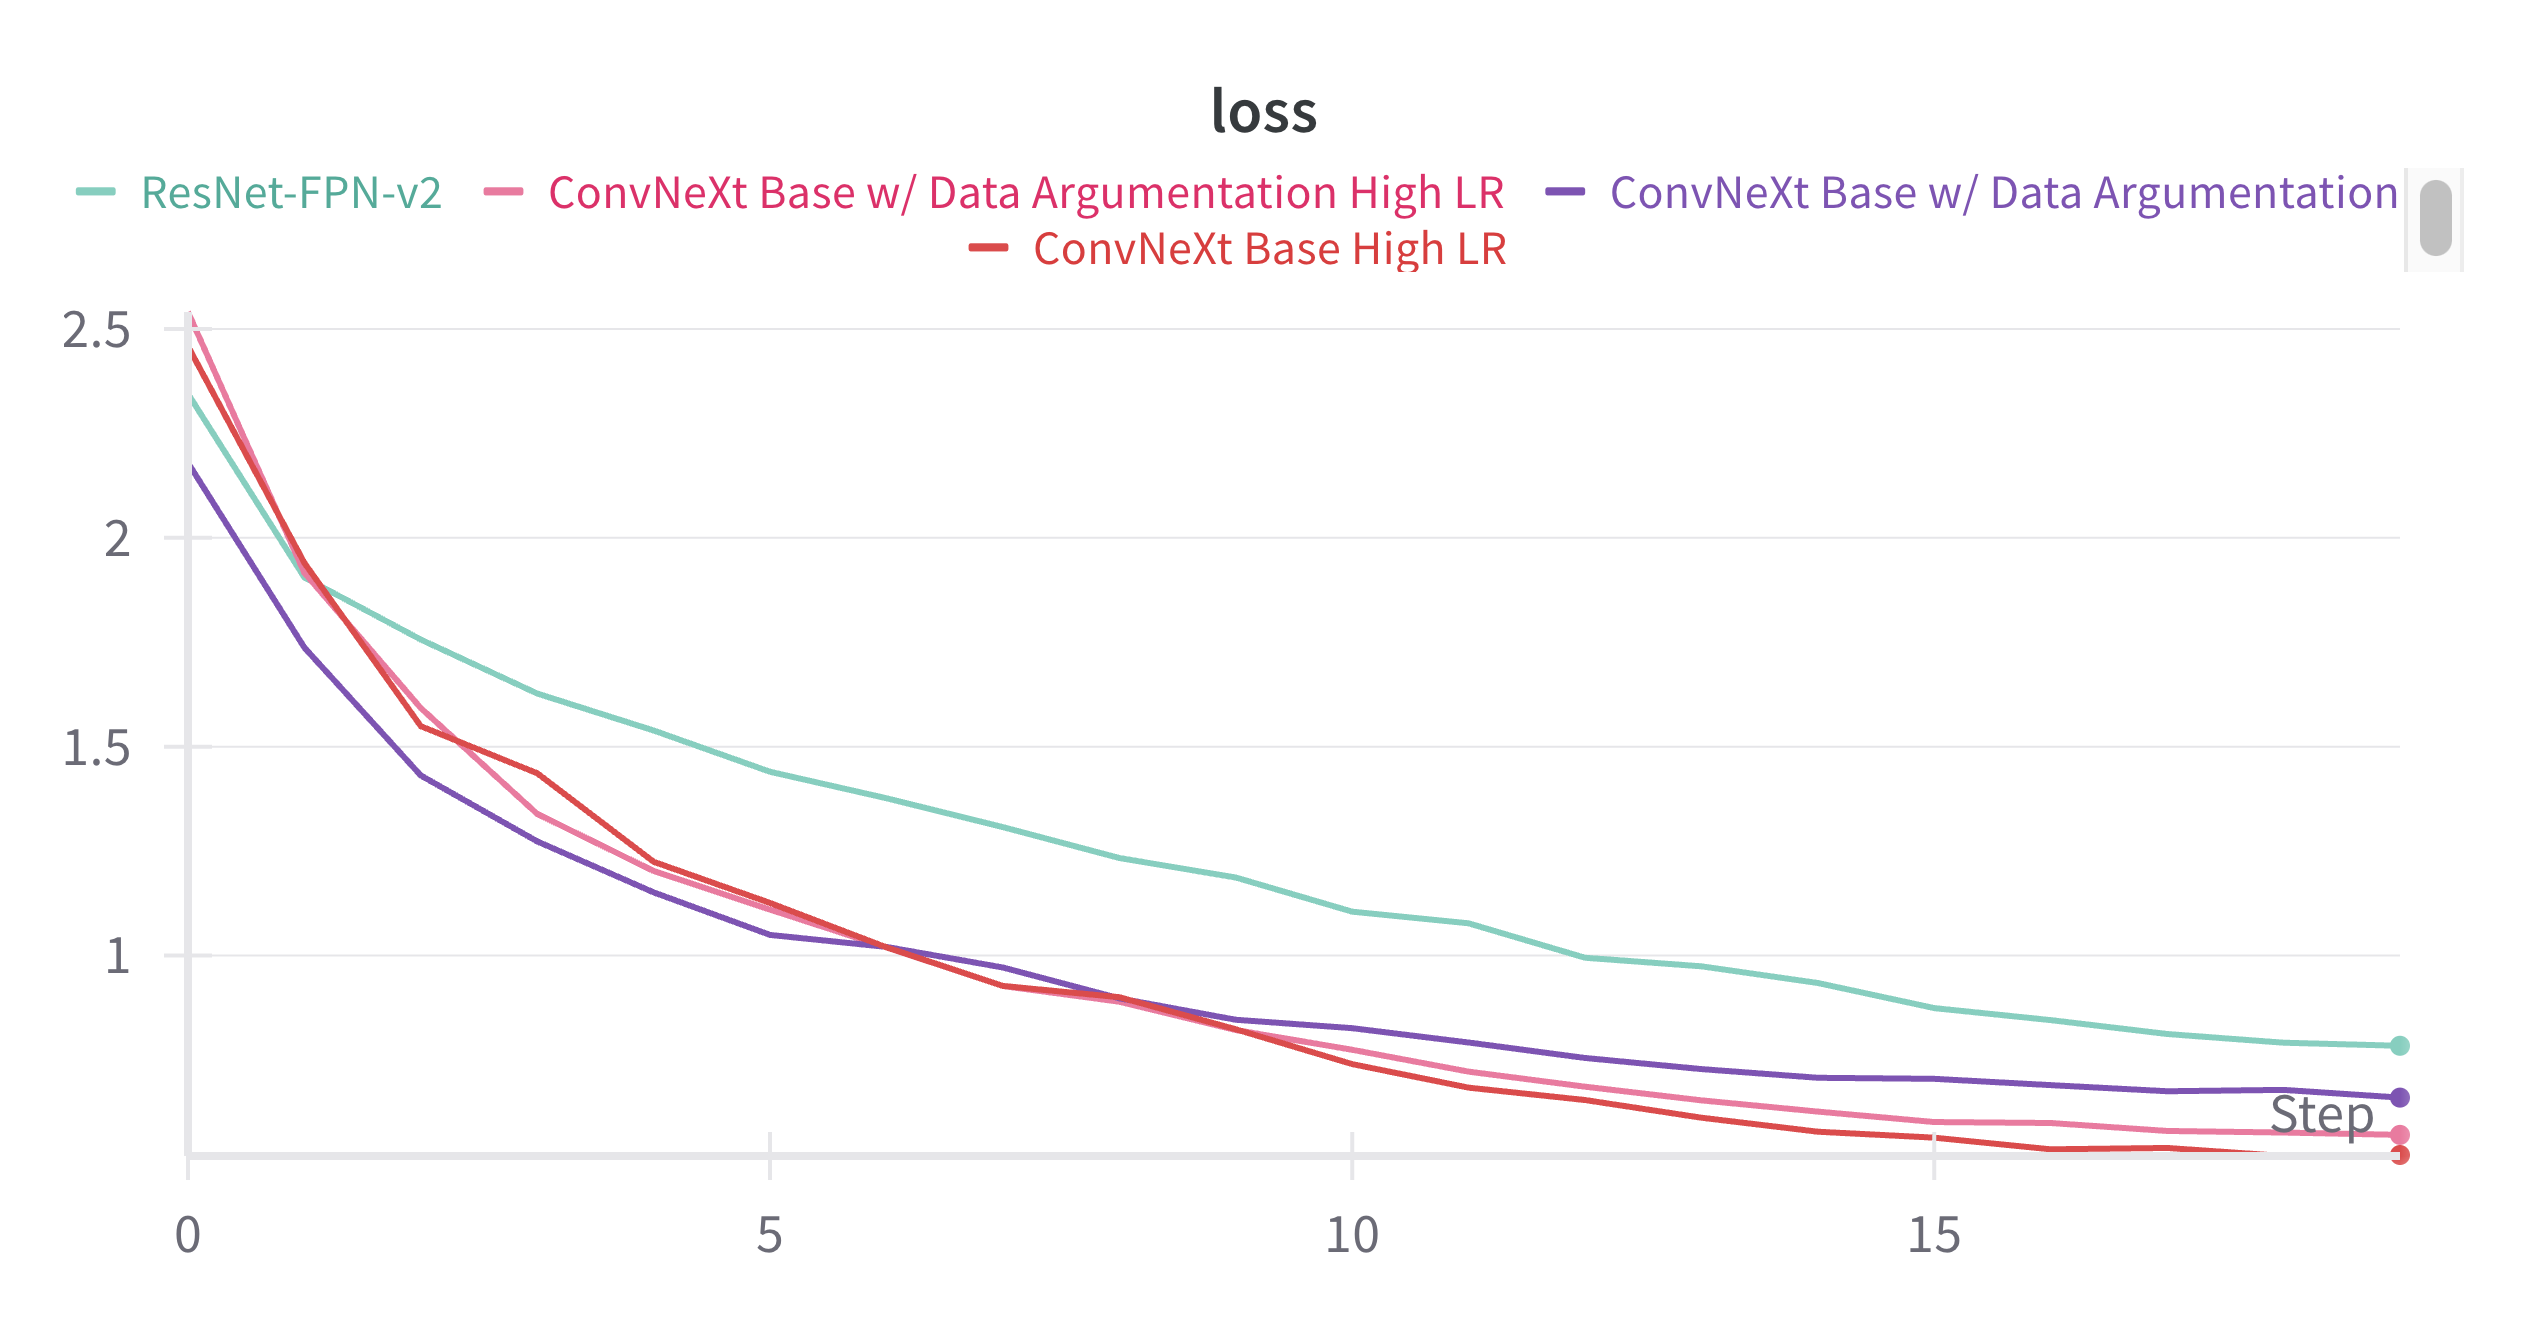
\includegraphics[width=0.95\linewidth]{figs/loss}
\caption{\textbf{Training loss evolution.} The plot shows the combined loss from RPN, classification, bounding box regression, and mask prediction components. The steady decrease indicates effective learning without significant oscillation, suggesting a stable optimization process.}
\label{fig:loss}
\end{figure}

\begin{figure}[H]
\centering
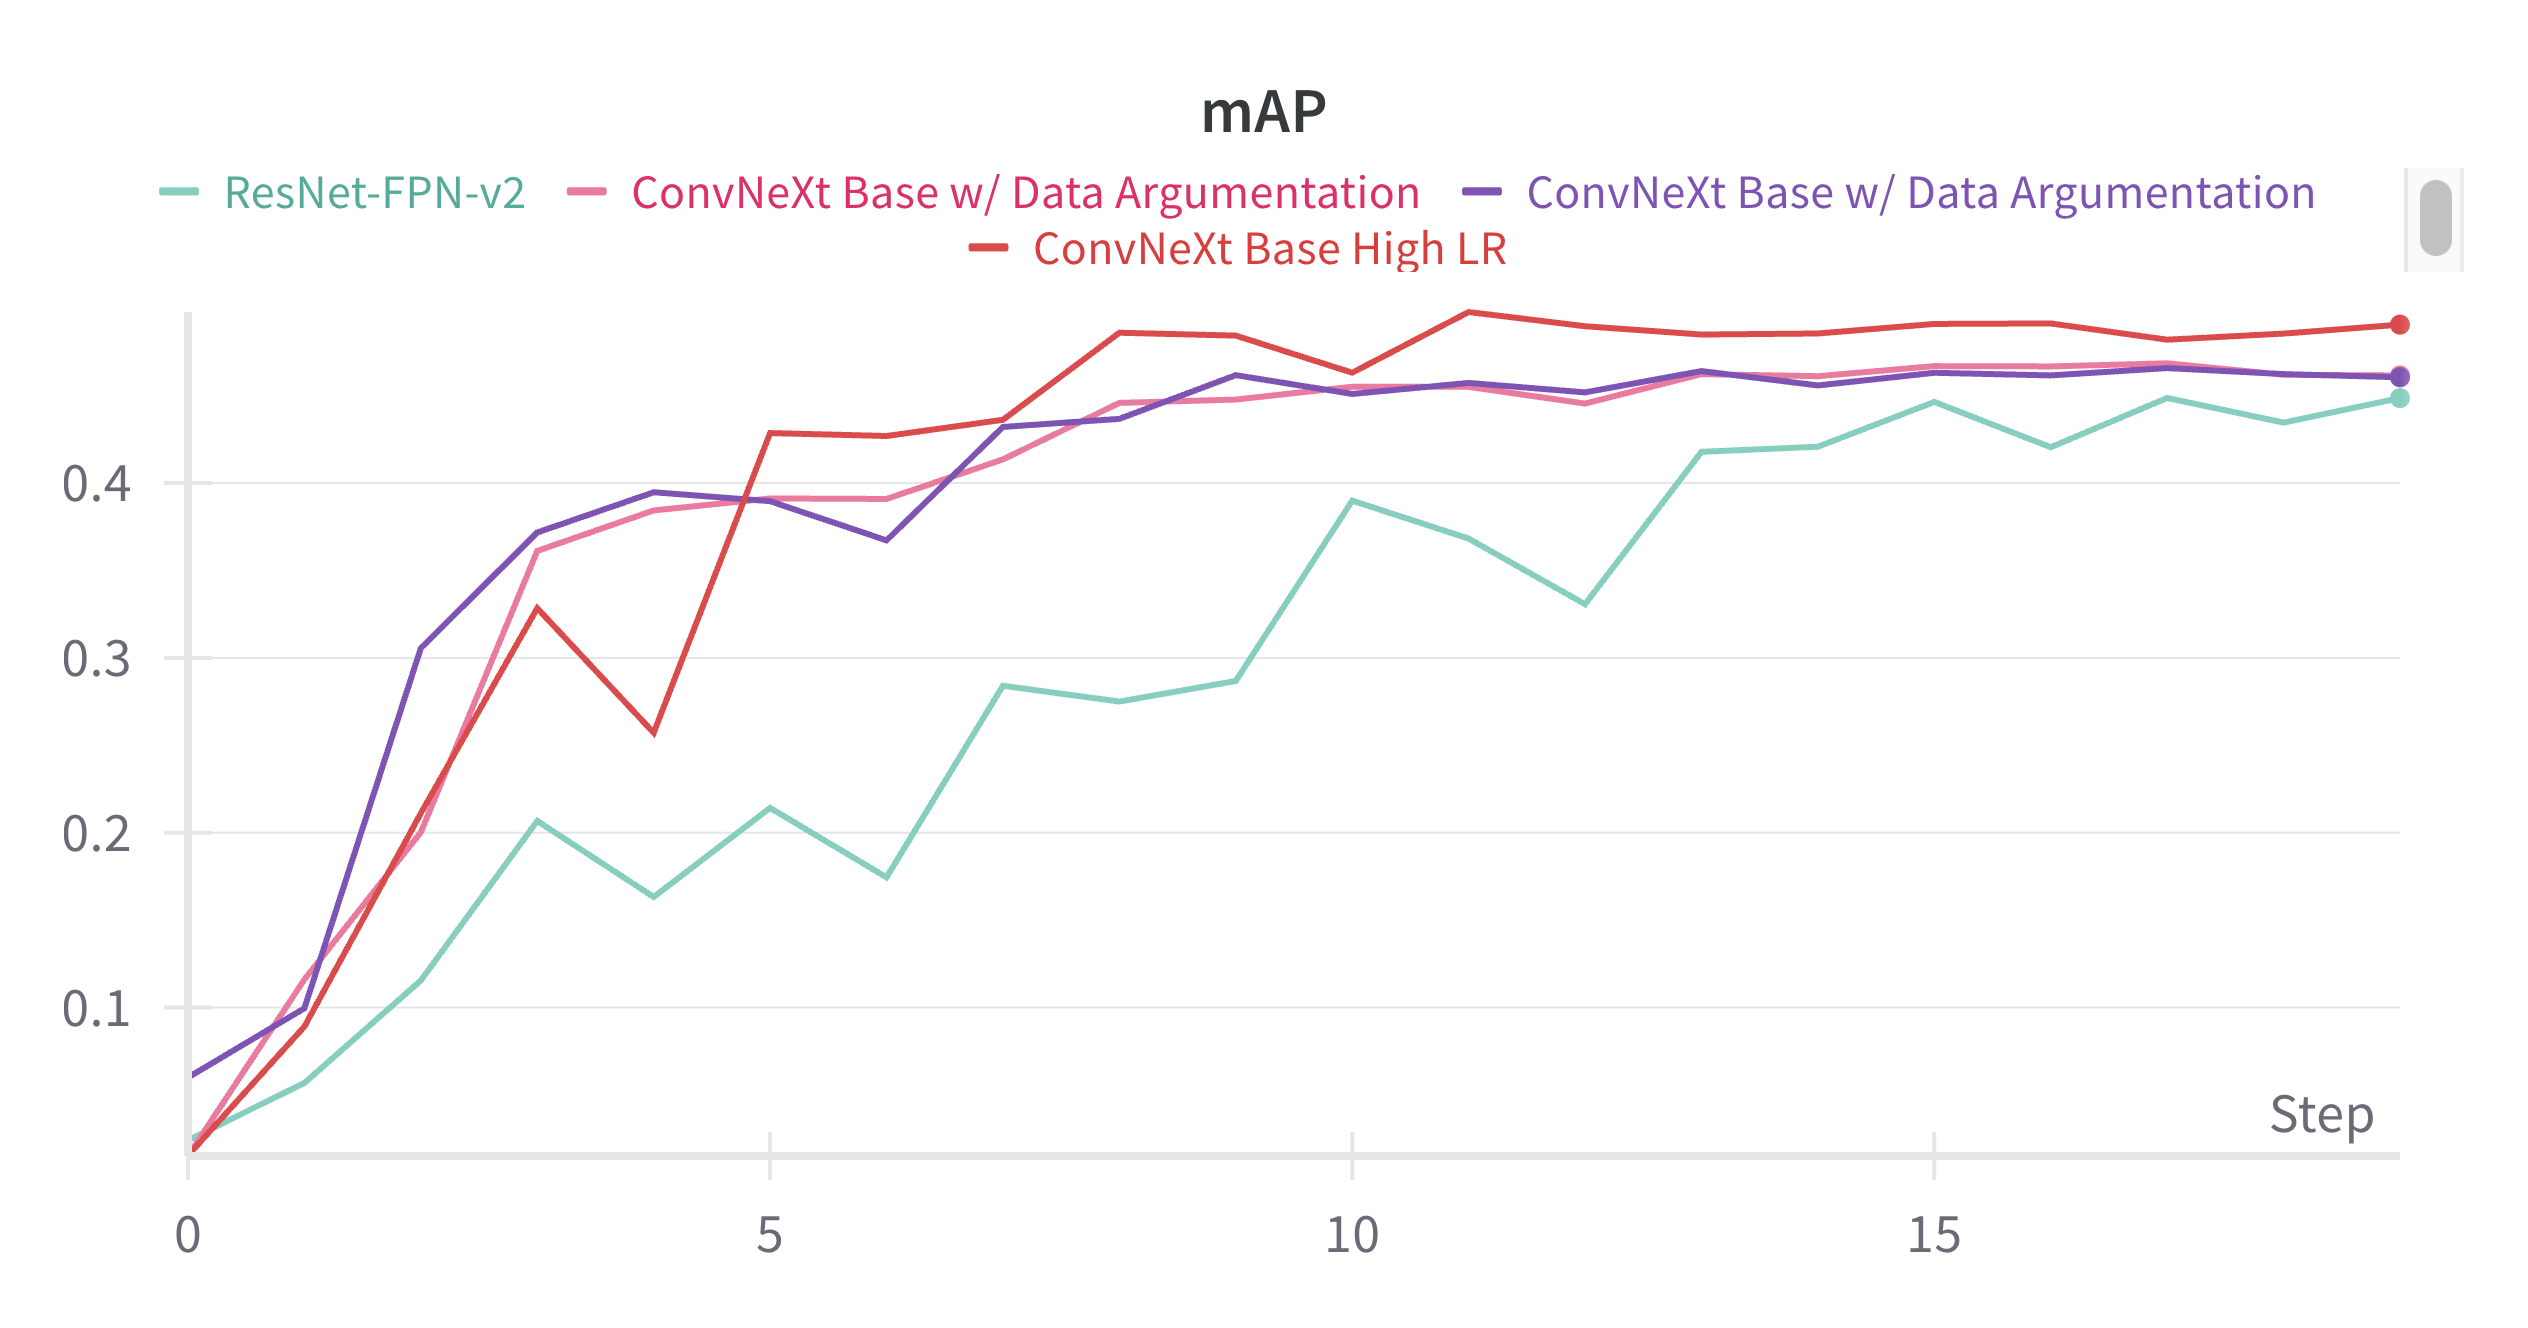
\includegraphics[width=0.95\linewidth]{figs/map}
\caption{\textbf{Mean Average Precision (mAP) across epochs.}}
\label{fig:map}
\end{figure}

\begin{figure}[H]
\centering
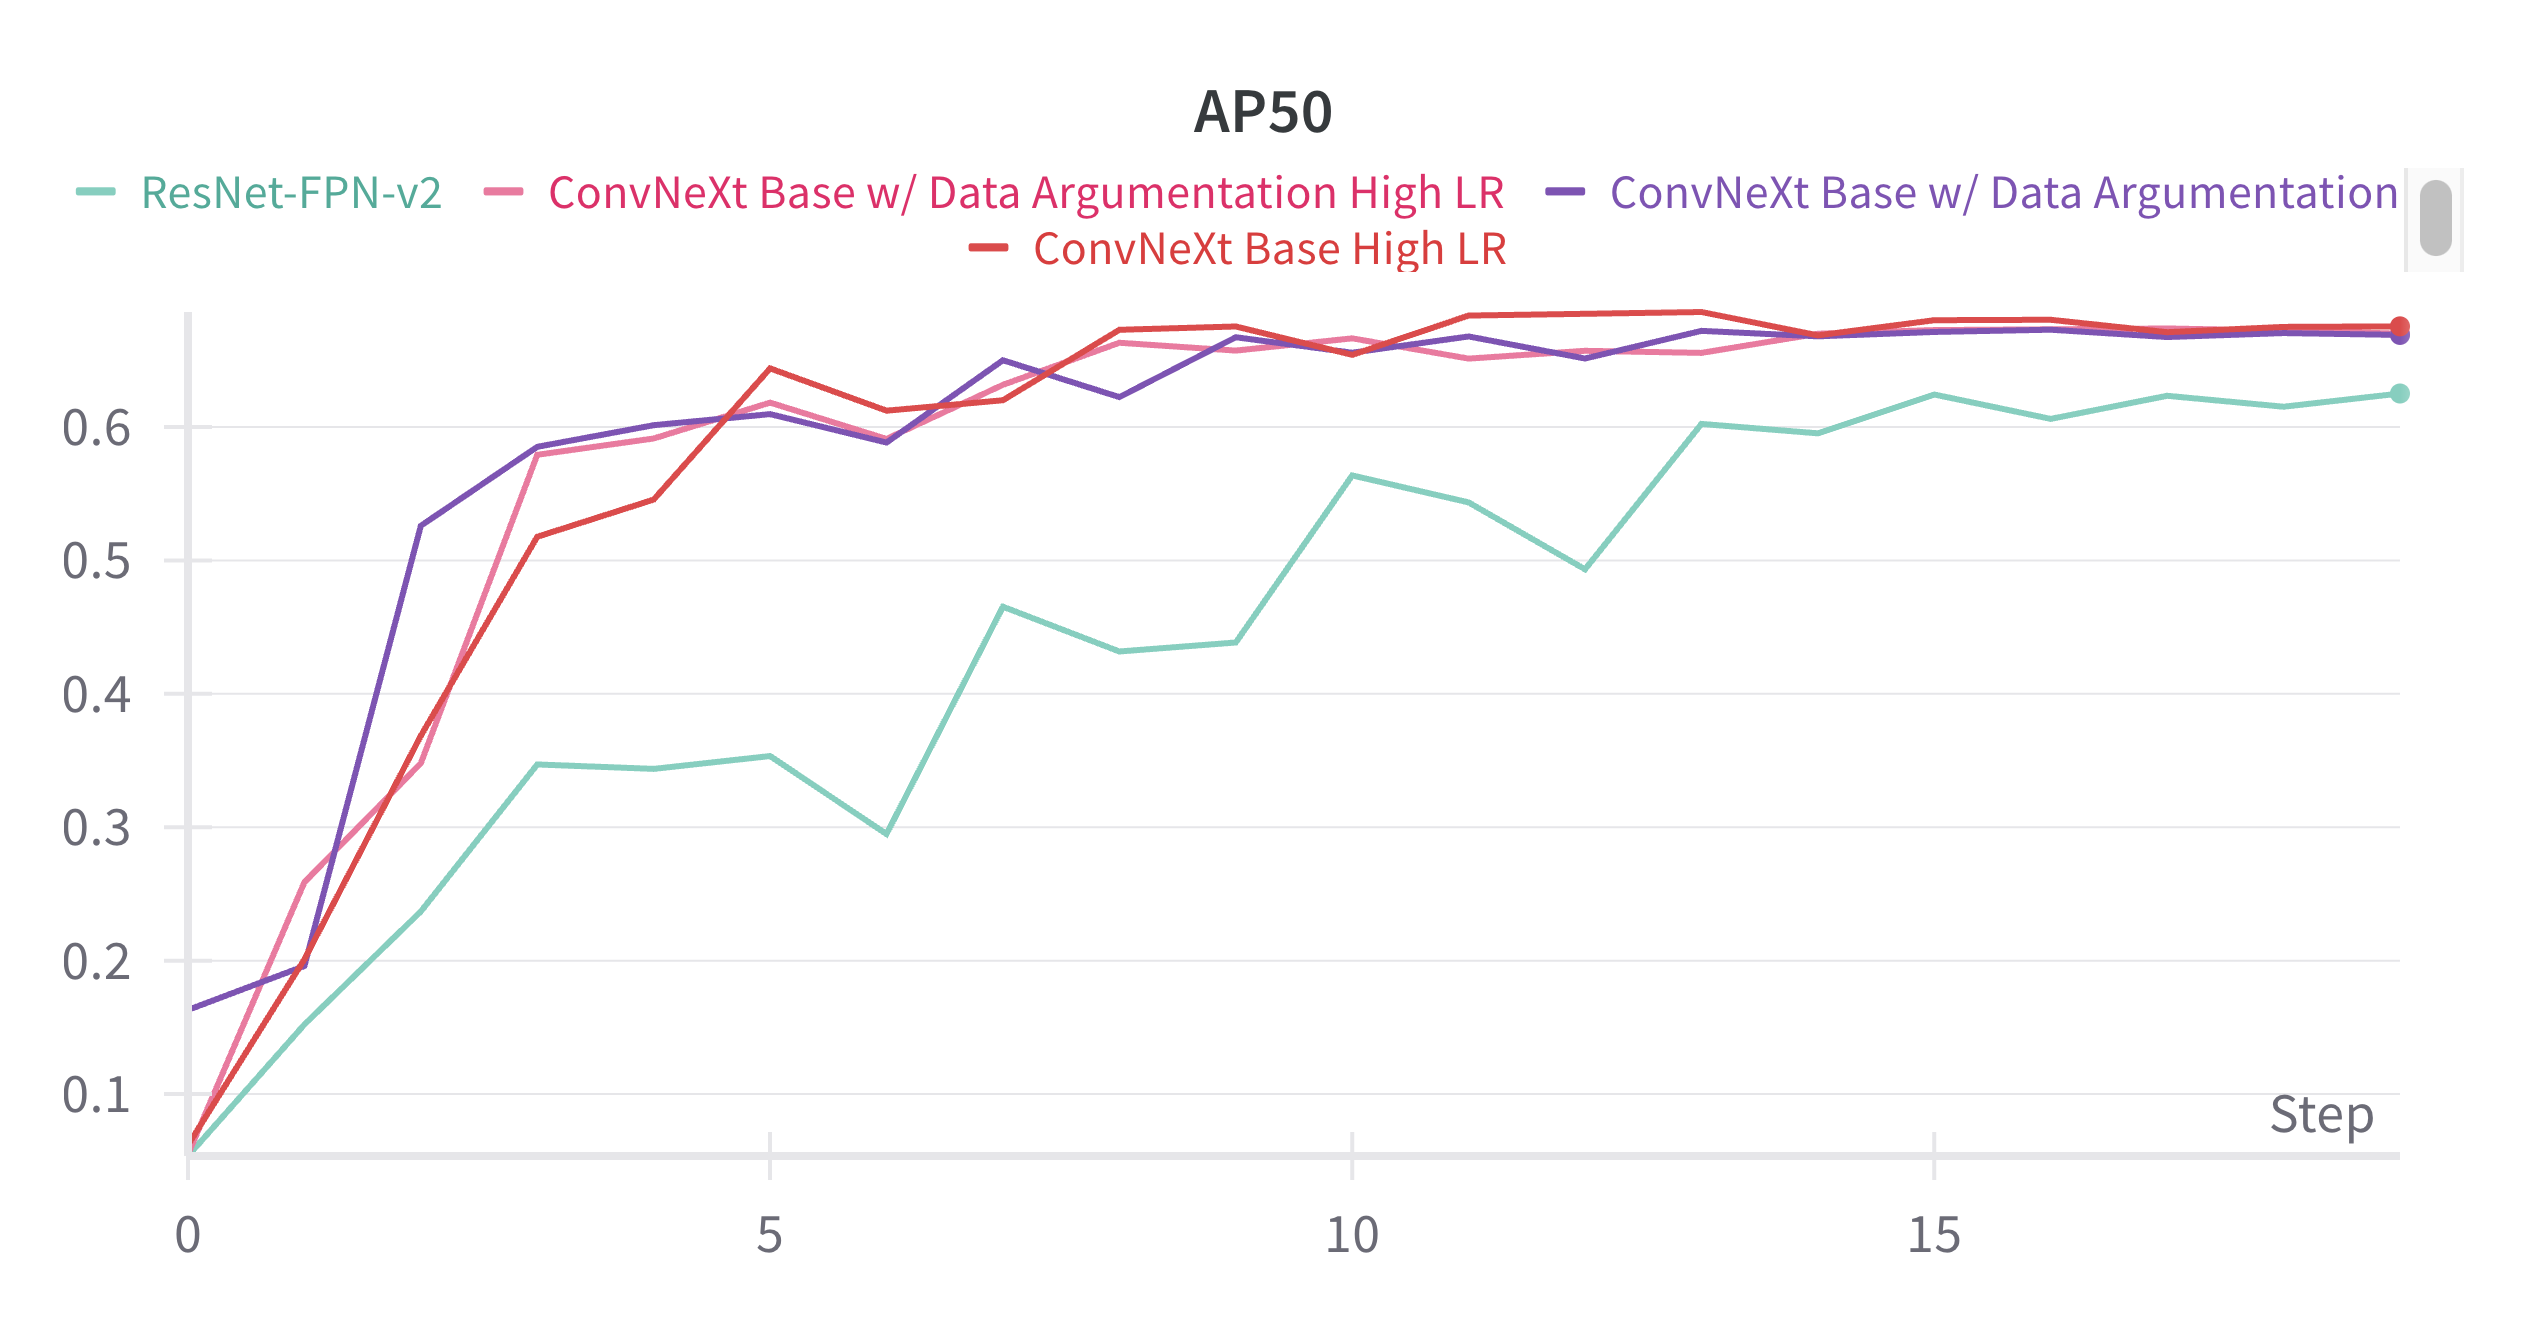
\includegraphics[width=0.95\linewidth]{figs/ap50}
\caption{\textbf{AP50 metric progression.}}
\label{fig:ap50}
\end{figure}

\begin{figure}[H]
\centering
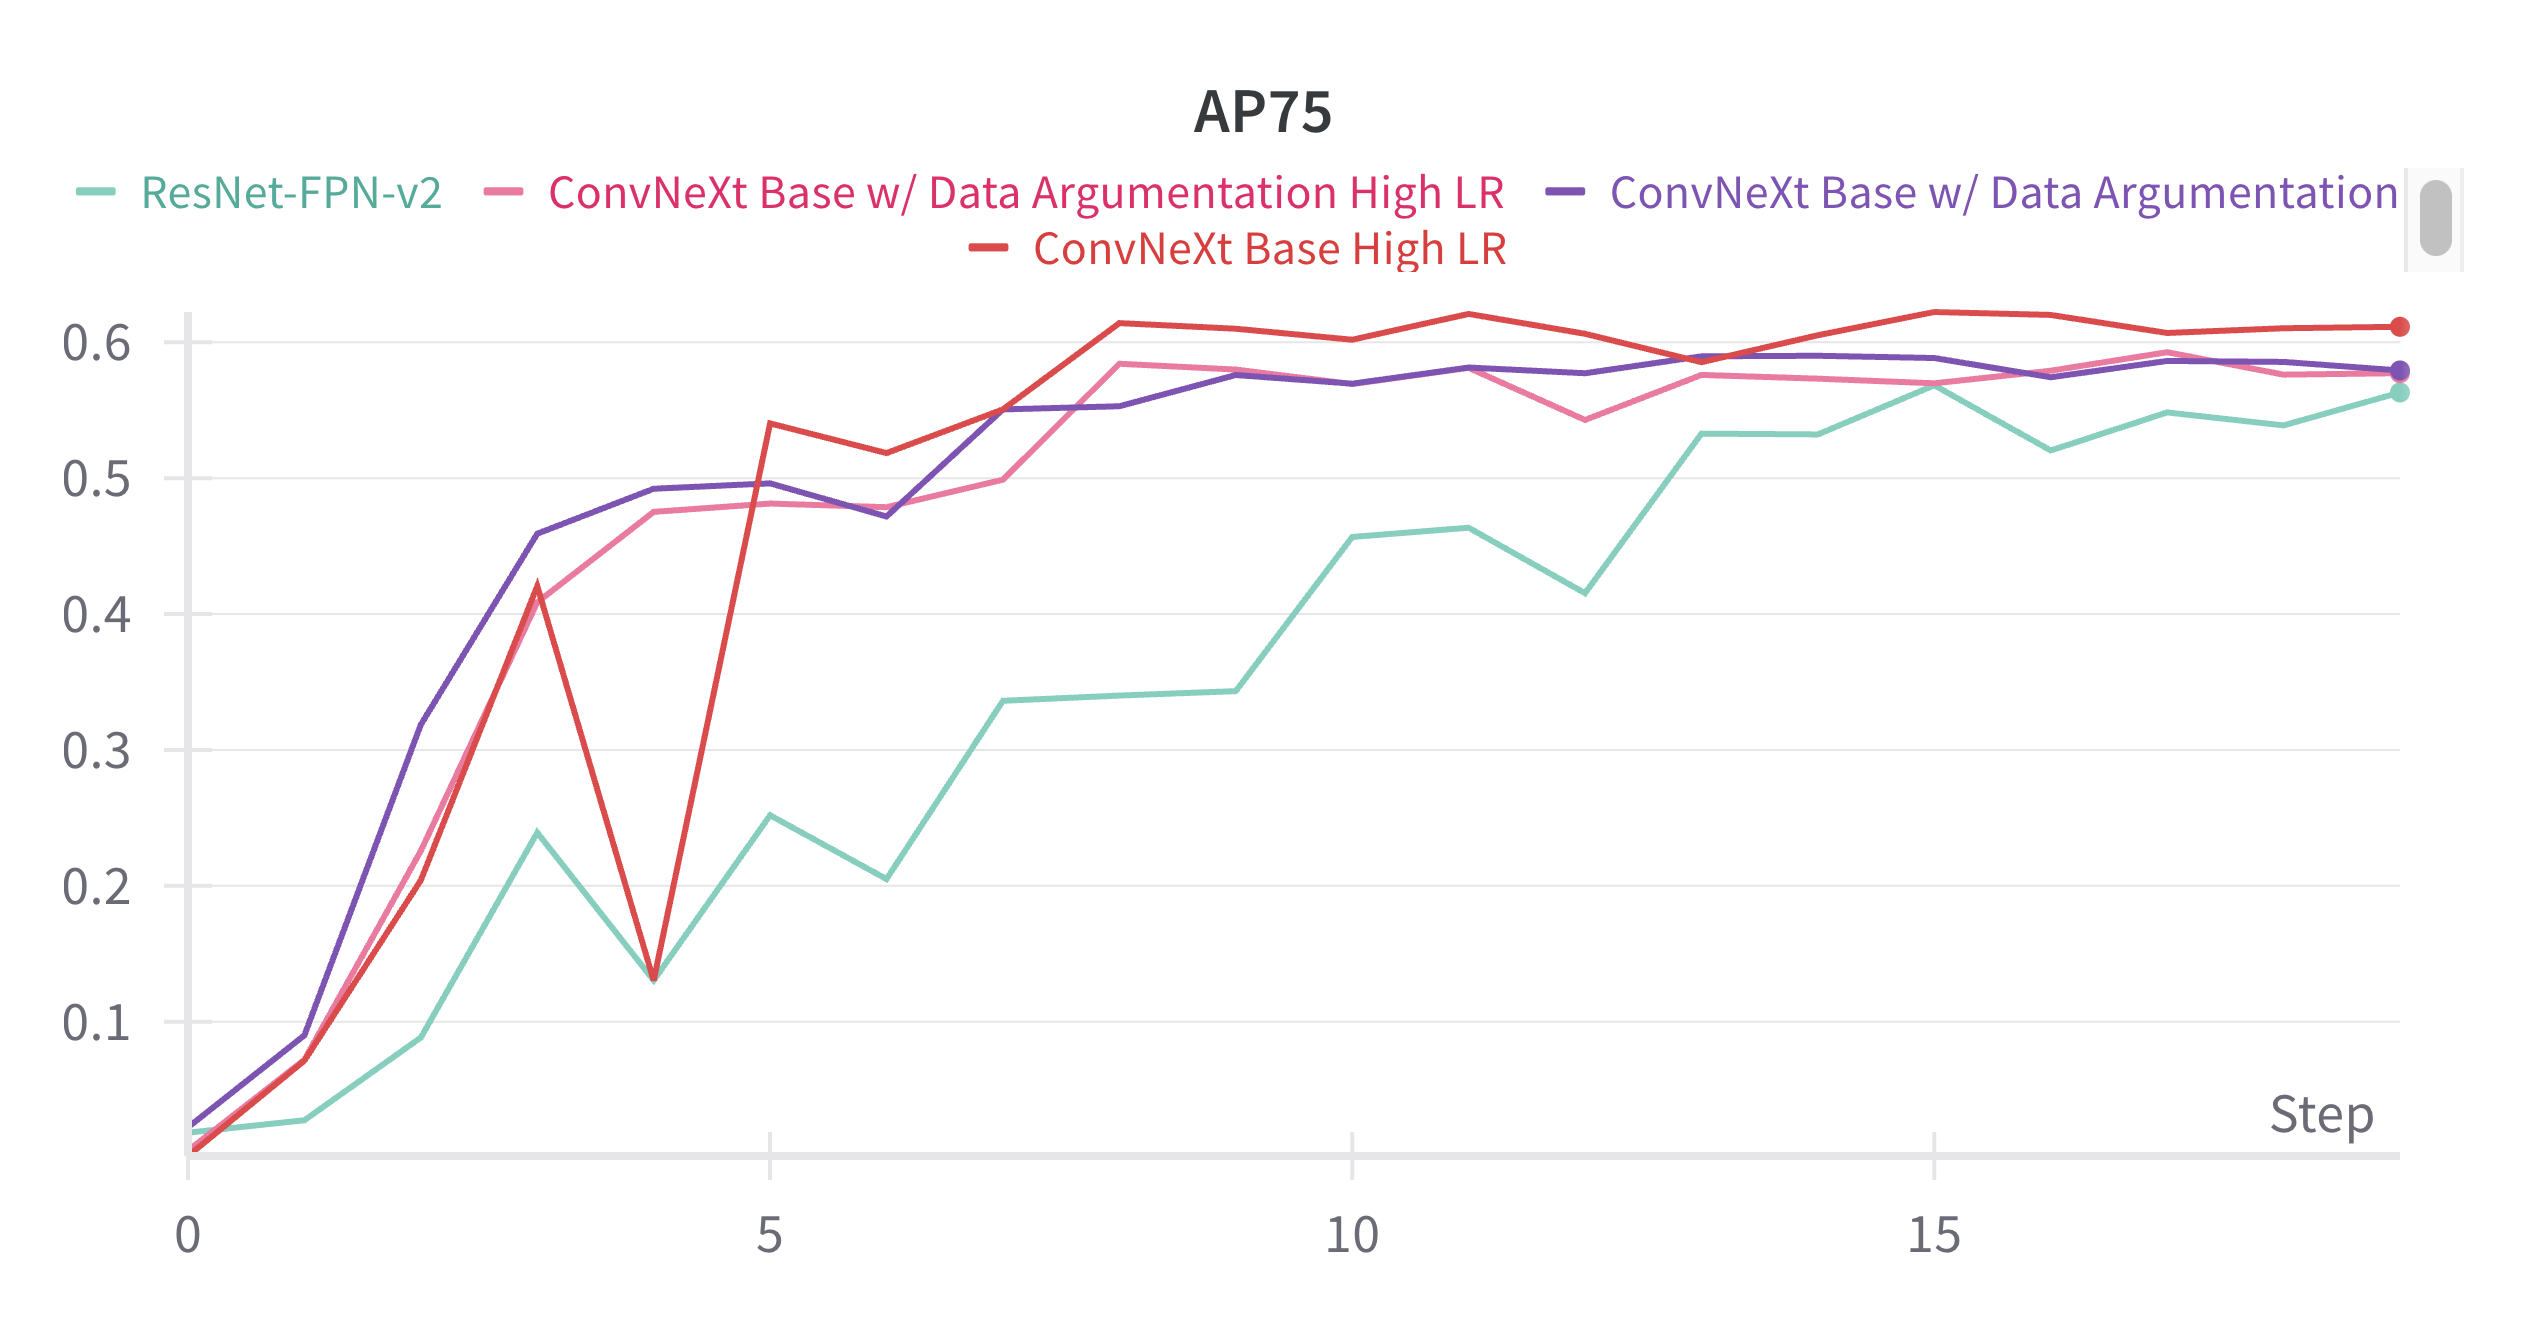
\includegraphics[width=0.95\linewidth]{figs/ap75}
\caption{\textbf{AP75 metric progression.}}
\label{fig:ap75}
\end{figure}

The training curves demonstrate consistent performance improvement across all metrics. The gap between AP50 and AP75 indicates that while the model successfully identifies most cell instances (high AP50), there remains room for improvement in precise boundary delineation (comparatively lower AP75).

\subsection{Ablation Studies}

\begin{table}[h]
\centering
\caption{\textbf{Impact of Different Components on Model Performance.} This table demonstrates the incremental improvements achieved through architectural and training strategy optimizations. The ConvNeXt-Base backbone with optimized learning rate achieves the best overall performance.}
\resizebox{\columnwidth}{!}{%
\begin{tabular}{lccc}
\toprule
\textbf{Configuration} & \textbf{mAP} & \textbf{AP50} & \textbf{AP75} \\
\midrule
ResNet-50 Baseline & 0.44863 & 0.62514 & 0.56307 \\
+ ConvNeXt-Base (1e-4) & 0.47720 & \textbf{0.68718} & 0.58521 \\
+ w/ Higher LR (3e-4) & \textbf{0.49063} & 0.68718 & \textbf{0.61138} \\
+ Advanced Augmentation & 0.46052 & 0.66906 & 0.57922 \\
\bottomrule
\end{tabular}%
}
\label{tab:ablation}
\end{table}

The ablation studies reveal several important insights:
\begin{enumerate}
\item Replacing the ResNet-50 backbone with ConvNeXt-Base provides a substantial performance boost across all metrics, with mAP increasing by nearly 3 percentage points.
\item Optimizing the learning rate from 1e-4 to 3e-4 further improves performance, particularly for the AP75 metric, suggesting better boundary precision.
\item Interestingly, while advanced augmentation was expected to improve performance, it showed slightly lower metrics. This suggests that for this particular cell dataset, the model benefits more from architectural improvements than from extensive data augmentation, possibly because the augmentations may introduce artifacts that don't reflect natural cell variations.
\end{enumerate}


\subsection{Public Score}

\begin{figure}[H]
\centering
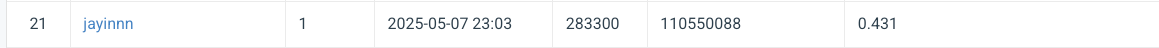
\includegraphics[width=0.95\linewidth]{figs/screenshot001}
\caption{\textbf{Public leaderboard performance.} The model achieved a public score of 0.431 on the test set.}
\label{fig:public score}
\end{figure}

\section{Discussion}

The ConvNeXt backbone proved to be substantially more effective than the standard ResNet-50 backbone for cell instance segmentation. The key advantages of ConvNeXt included better feature extraction, especially for the fine boundary details critical in cell segmentation tasks. The locality bias inherent in ConvNeXt's design helped preserve spatial details important for segmenting individual cells that may be touching or overlapping.

The ablation studies reveal an interesting finding: while the advanced backbone architecture significantly improved performance, the advanced augmentation techniques showed mixed results. This suggests that for cell segmentation, architectural improvements may yield more substantial benefits than data augmentation alone.

The learning rate optimization proved crucial, with the higher learning rate of 3e-4 demonstrating superior performance compared to the more conservative 1e-4 setting. This suggests that with the limited dataset size, a more aggressive optimization approach allows the model to better explore the parameter space before convergence.

The relatively smaller gap between AP50 and mAP compared to typical object detection tasks indicates that the model is performing well at localizing cell boundaries precisely, which is essential for biological analysis applications where exact cell morphology is important.


In conclusion, this work demonstrates that even with a limited dataset of approximately 209 images, advanced architectures like ConvNeXt combined with carefully designed training strategies can achieve strong performance on instance segmentation tasks for medical cell images. The approach presented here not only achieves competitive results but also provides insights into the relative importance of different components in cell segmentation pipelines.

\section{GitHub Link}
\noindent\url{https://github.com/jayin92/NYCU-VRDL-HW3}


\bibliographystyle{plain}
\bibliography{main}



\end{document}
